Figuren ~\ref{degform} Visar en degform för manuell fyllning av en Ravioli. Den fungerar genom att man lägger en Raviolideg på formen, efter detta läggs fyllningsmaterial på degen och sist tillsluter man degen genom att pressa formens handtag mot varandra. Degformen kan tillämpas att sluta degen automatiskt med hjälp av motorer. Lämpliga typer av motorer  är likströms- eller stegmotor.
\begin{figure}[h]
	\begin{center}
		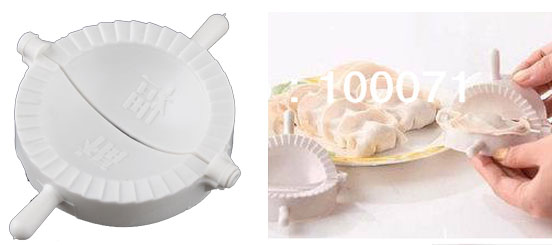
\includegraphics[scale=0.75]{images/ravioli_mould_trimed_1.jpg}
		\caption{Degform för manuell fyllning av en Ravioli}
		\label{degform}
	\end{center}
\end{figure}
\textbf{Likströmsmotor}\\*
Likströmsmotorer är den vanligaste motor som sitter i många olika produkter som leksaker, dataspel mm\cite{likstromsmotor}. Strömmen som en likströmsmotor förbrukar beror på belastningen. Denna egenskap kan användas som en sensor för att identifiera t.ex. hinder och i detta fall när degformen har pressat Raviolidegen nog för att tillsluta den.\\

\textbf{Stegmotor}\\*
Den här typen av motor liknar likströmsmotor men den skiljer sig från likströmsmotor genom en unik egenskap: stegmotor roterar ett steg vid en strömpuls. Steget minskar med ökat antal poler i statorn. Genom att beräkna antal pulsar som skickas till steg-motorn, kan man exakt positionera ett objekt \cite{stegmotor}.
